\documentclass[../manuscript.tex]{subfiles}

\section{Введение}

Секвенирование одиночных клеток на протяжении последних нескольких лет было одной из самых горячих тем в науке: single-cell технологии дважды получали звание "method of the year" по версии Nature Methods\cite{MethodOfTheYear2013}\cite{MethodOfTheYear2019}, а 10X Genomics, основная компания-производитель оборудования для single-cell секвенирования, заняла 69 строчку в рейтинге 500 наиболее быстрорастущих компаний США\footnote{https://www.inc.com/inc5000/2019/top-private-companies-2019-inc5000.html}. Возможность изучать биологические процессы в тканях на уровне отдельных клеток привела к прорывным открытиям во многих областях науки\cite{SingleCellRevolution}\cite{SingleCellComingOfAge}, особенно в персонализированной онкологии\footnote{https://www.nature.com/articles/d42473-019-00310-5}. В частности, в задаче восстановления клональной структуры опухоли — определения групп клеток, имеющих схожий набор индуцированных генетических мутаций. Понимать состав опухоли критически важно для подбора лечения, особенно в высокоинвазивных раках с высокой частотой мутаций. 

\begin{figure}[H]
	\centering
	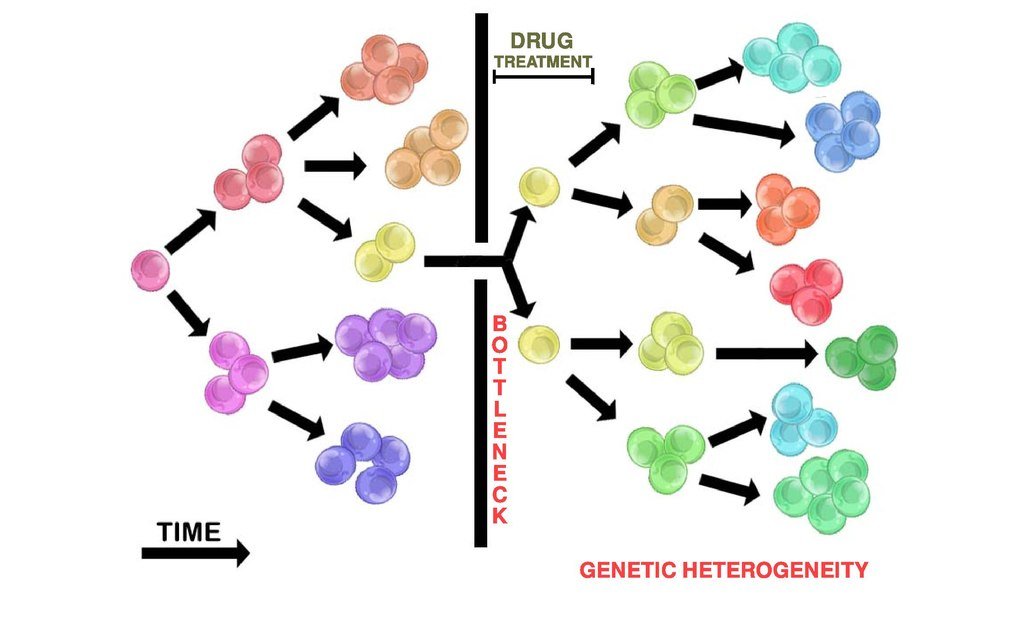
\includegraphics[keepaspectratio=true, scale=0.4]{images/tumour_heterogeneity_treatment_bottleneck.jpg}
	\caption{При подборе терапии нужно учитывать клональный состав опухоли. Лечение может убивать некоторые клональные линии, но не действовать на остальные, из-за чего случается рецидив.}
\end{figure}

В данной дипломной работе рассматривается байесовский подход к этой задаче. В ней предложен алгоритм байесовского машинного обучения XClone — графическая статистическая модель опухолевых образцов. В её задачи входит не только анализ клонального состава образца, но и поиск аллель-специфических структурных мутаций, по которым можно пронаблюдать эволюцию опухоли. Алгоритм XClone развивает идеи, заложенные доктором Янхуа Хуань в статьях "Cardelino"\cite{Cardelino} и "Vireo"\cite{Vireo}. На концептуальном уровне, XClone также можно использовать для интеграции геномных и транскриптомных данных, но на данный момент, в силу низкого разрешения данных РНК-секвенирования одиночных клеток, хорошие результаты в этом направлении были получены только на синтетических данных. Метод был опробован на реальных данных, извлечённых из медуллобластомы — детской опухоли мозга, — полученных по протоколам компаний 10X Genomics и Smart-Seq, но концептуально он не привязан к конкретной платформе и может быть адаптирован к другим форматам входных данных. 


Текущая  версия XClone состоит из двух основных частей, связанных расстановкой клональных меток. 

Первая часть получила название "RDR-модуль", где RDR расшифровывается как "read depth ratio", отношение наблюдаемой доли числа прочтений внутри фиксированного сегмента генома к ожидаемой. В теоретических моделях ДНК-секвенирования, где предполагается равномерное распределение прочтений по геному, RDR должно стремиться к реальному числу копий этого сегмента пополам. Это основная величина, на которую опираются алгоритмы поиска структурных вариаций генома, в том числе CellRanger от 10X Genomics и CHISEL\cite{ChiselBiorxiv}.

Вторая часть носит название "ASE-модуль", где ASE означает "allele-specific expression". Эта часть модели позволяет не только понять, сколько копий сегмента образовалось в процессе онкогенеза, но и сколько из этих копий лежит на каждой конкретной хромосоме. Важность этой информации была обоснова во многих статьях по онкологии. 10,33–35. For example, copy-neutral loss of heterozygosity (LOH) – where one allele is lost and the other duplicated so the total copy number remains 2 – is common in many cancers 33,36–41. Allele-specific copy numbers have also been shown to be essential for accurate inference of whole-genome duplications (WGDs)24,42 and timing WGDs relative to other CNAs10,24,43. Despite the demonstrated importance of allele-specific copy numbers, previous single-cell sequencing studies have assumed that low-coverage data is too shallow to obtain allele-specific information from single cells7,8,44–46. Existing methods for identifying CNAs from single-cell sequencing data6–8,45–50 are limited to the inference of total copy number, which indicates only the sum of copy numbers at each locus, by analyzing differences between the observed and expected number of sequencing reads aligned to a locus, or the read-depth ratio (RDR). The signal to detect allele-specific copy numbers is the B-allele frequency (BAF), or relative proportions of reads from the two alleles of a genomic region; however, standard methods to calculate the BAF from individual germline heterozygous SNPs do not work with extremely low coverage sequencing data.

По состоянию на июнь 2020 года, опубликован только один непосредственный аналог XClone — алгоритм CHISEL\cite{ChiselBiorxiv}, разработанный в лаборатории Бена Рафаэля в Принстонском университете. CHISEL был выложен на онлайн-архив предпубликаций bioRxiv уже после того, как была начата работа над XClone. Тем не менее, несмотря на то, что оба метода дают сравнимые результаты в задаче поиска аллель-специфических структурных вариаций, XClone выгодно отличается от CHISEL тем, что в его статистическую модель можно естественным образом интегрировать другие типы данных, такие как данные РНК-секвенирования, данные о соматических мутациях, данные о митохондриальной ДНК, в то время как алгоритм CHISEL решает узкую задачу и никаким тривиальным образом не обобщается. Авторы верят, что именно в этой гибкости и масштабируемости заключается научная новизна XClone.


